\documentclass{article}
\usepackage{v-test-paper}
\title{\textsc{Unit \& Dimensions}}
\date{February 22, 2024}

\newcommand{\itemstared}{\refstepcounter{enumi}\item[$^\star$\theenumi.]}
\usetikzlibrary{matrix,  positioning, patterns, backgrounds}
\renewcommand{\ans}{\quad}


\tikzstyle{root} = [rectangle, rounded corners, 
minimum width=3cm, 
minimum height=0.7cm,
text centered, 
draw, 
font=\scshape,
]
\tikzstyle{child} = [rectangle, rounded corners, 
inner sep=2mm,
text centered, 
draw, 
font=\itshape,
text width=3.25cm,
]

\tikzstyle{child-branch} = [
    rectangle, 
    rounded corners, 
    inner sep=2mm,
    text centered, 
    draw, 
    font=\itshape,
    text width=2.5cm,
    level distance=5mm,
]



\tikzstyle{arrow} = [thick,->,>=latex]


\begin{document}
\maketitle
\begin{center}
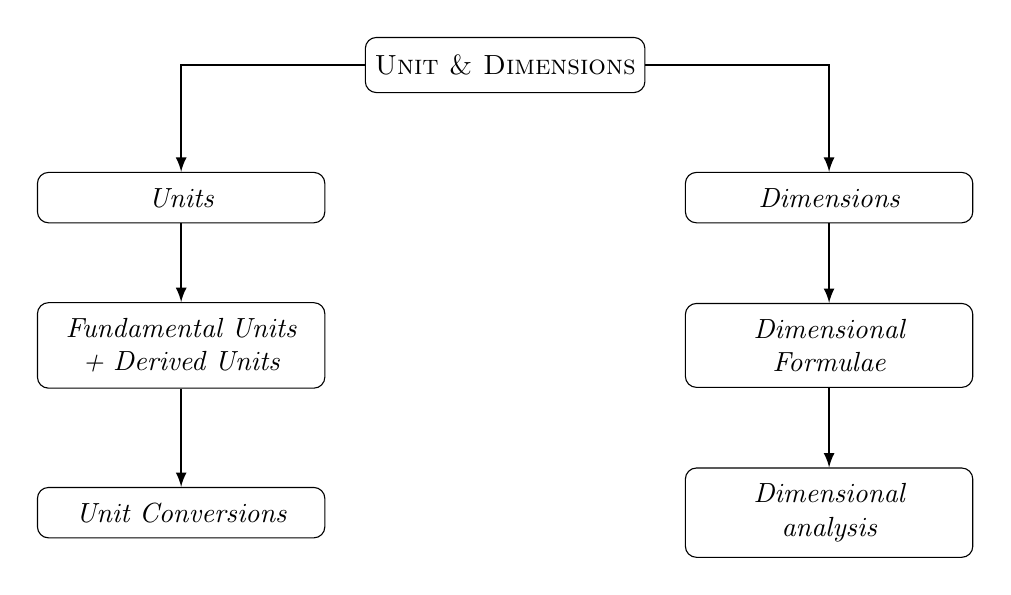
\begin{tikzpicture}[node distance=2cm]

\matrix [column sep=5mm,row sep=10mm]
{
&\node (root) [root] {Unit \& Dimensions};\\
\node (child-left)[child] {Units}; & &
\node (child-right)[child] {Dimensions}; \\
\node (child-left-b)[child] {Fundamental Units + Derived Units}; & &
\node (child-right-b)[child] {Dimensional Formulae}; \\
\node (child-left-bb)[child] {Unit Conversions}; & &
\node (child-right-bb)[child]{Dimensional analysis};\\
};

\draw [arrow] (root) -| (child-left);
\draw [arrow] (root) -| (child-right);
\draw [arrow] (child-left) --(child-left-b);
\draw [arrow] (child-right) -- (child-right-b);
\draw [arrow] (child-right-b) -- (child-right-bb);
\draw [arrow] (child-left-b)--(child-left-bb);
\end{tikzpicture}
\end{center}

\begin{center}
    \textsc{Problems}
\end{center}
\begin{enumerate}
    \item The equation of a wave travelling on a string stretched along the x-axis is given by \[ y=Ae^{-\left(\dfrac{x}{a}+\dfrac{t}{T}\right)^2} \] Which of the following is the dimension of $A, a, \text{ and } T$ respectively?
        \begin{tasks}(2)
            \task $[L], [L], [T]$ \ans
            \task $[L], [T], [L]$
            \task $[T], [L], [L]$
            \task $[L], [T], [T]$
        \end{tasks}

    \item A dimensionless quantity
        \begin{tasks}(2)
            \task never has a unit
            \task may have a unit \ans
            \task always has a unit
            \task does not exist
        \end{tasks}

    \item Let $x$ and $a$ stand for distance. In the equation \[ \int \dfrac{\d{x}}{\sqrt{2ax-x^2}} = a^n \sin^{-1}\left(\dfrac{x}{a}-1\right) \] The value of $n$ for which the equation is dimensionally correct is
        \begin{tasks}(4)
            \task 0\ans
            \task 1
            \task 2
            \task 3
        \end{tasks}

    \item Which of the following combinations has the dimension of electrical resistance($\varepsilon_0$ is the permittivity of vacuum and $\upmu_0$ is the permeability of vacuum)?
    \begin{tasks}(2)
        \task $\sqrt{\dfrac{\upmu_0}{\varepsilon_0}}$\ans
        \task $\dfrac{\upmu_0}{\varepsilon_0}$
        \task $\sqrt{\dfrac{\varepsilon_0}{\upmu_0}}$
        \task $\dfrac{\varepsilon_0}{\upmu_0}$
    \end{tasks}

    \item In the formula $X=5YZ^2$, $X$ and $Z$ have dimensions of capacitance and magnetic field respectively. What are the dimensions of $Y$ in SI units?
        \begin{tasks}(2)
            \task $[M^{-1}L^{-2}T^4A^2]$
            \task $[M^{-2}L^{0}T^{-4}A^{-2}]$
            \task $[M^{-3}L^{-2}T^8A^4]$\ans
            \task $[M^{-2}L^{-2}T^6A^3]$
        \end{tasks}

    \item Let $l, r, c,$ and $\nu$ represent inductance, resistance, capacitance, and voltage respectively. The dimension of $\dfrac{l}{rc\nu}$ in SI units will be
    \begin{tasks}(2)
        \task $[LT^2]$
        \task $[LTA]$
        \task $[A^{-1}]$\ans
        \task $[LA^{-2}]$
    \end{tasks}

    

    

    \item Match the two columns
    \renewcommand{\arraystretch}{1.5}
    \begin{table}[h]
        \begin{center}
        \begin{tabular}{p{5cm}|p{3cm}}
        \hline
        Column I & Column II \\
        \hline
        (a) Boltzmann constant & (p) $[ML^2T^{-1}]$ \\
        (b) Coefficient of viscosity & (q) $[ML^{-1}T^{-1}]$ \\
        (c) Planck's constant & (r) $[MLT^{-3}K^{-1}]$ \\
        (d) Thermal conductivity & (s) $[ML^2T^{-2}K^{-1}]$ \\
        \hline
        \end{tabular}
        \end{center}
        \end{table}
        \begin{tasks}(2)
            \task $a \rightarrow p, b \rightarrow q, c \rightarrow r, d \rightarrow s$
            \task $a \rightarrow s, b \rightarrow q, c \rightarrow p, d \rightarrow r$ \ans
            \task $a \rightarrow r, b \rightarrow s, c \rightarrow p, d \rightarrow q$
            \task $a \rightarrow p, b \rightarrow s, c \rightarrow q, d \rightarrow r$
        \end{tasks}

    \item Match the physical quantities given in Column I with dimensions expressed in terms of mass
    (M), length (L), time (T), and charge (Q) given in Column II.
        \begin{table}[h]
            \begin{center}
            \begin{tabular}{p{5cm}|p{3cm}}
            \hline
            Column I & Column II \\
            \hline
            (a) Angular momentum & (p) $[ML^3T^{-2}]$ \\
            (b) Latent heat & (q) $[ML^{2}Q^{-2}]$ \\
            (c) Torque & (r) $[ML^2T^{-1}]$ \\
            (d) Capacitance & (s) $[ML^3T^{-1}Q^{-2}]$ \\
            (e) Inductance & (t) $[M^{-1}L^{-2}T^{2}Q^{2}]$ \\
            (f) Resistivity & (u) $[L^2T^{-2}]$ \\
            \hline
            \end{tabular}
            \end{center}
        \end{table}
        \begin{tasks}(2)
            \task $a \rightarrow r, b \rightarrow u, c \rightarrow p, d \rightarrow t, e \rightarrow q, f \rightarrow s$\ans
            \task $a \rightarrow r, b \rightarrow p, c \rightarrow q, d \rightarrow s, e \rightarrow t, f \rightarrow u$
            \task $a \rightarrow p, b \rightarrow q, c \rightarrow r, d \rightarrow s, e \rightarrow u, f \rightarrow t$
            \task $a \rightarrow q, b \rightarrow p, c \rightarrow r, d \rightarrow t, e \rightarrow s, f \rightarrow u$
        \end{tasks}

        

    \item The force of interaction between two atoms is given by \[ F=\alpha \beta e^{-\left(\dfrac{x^2}{\alpha k T}\right)} \] where $x$ is the distance, $k$ is the Boltzmann constant and $T$ is the temperature and $\alpha, \beta$ are constants. The dimensions of $\beta$ is 
    \begin{tasks}(2)
        \task $[ML^2T^{-2}]$
        \task $[MLT^{-2}]$
        \task $[MLT^{-1}]$
        \task $[M^2LT^{-4}]$\ans
    \end{tasks}

    \item Taking force(F), length(L) and time(T) to be the fundamental quantities find the dimensions of energy.
    \begin{tasks}(2)
        \task $[F^2LT]$
        \task $[FL^2T^{-2}]$
        \task $[FL]$\ans
        \task $[FL^2T^{-1}]$
    \end{tasks}

\end{enumerate}


\pagebreak

\begin{center}
\texttt{Answer Key}
\begin{multicols}{5}
\begin{enumerate}
\item (b)
\item (b)
\item (a)
\item (b)
\item (d)
\item (b)
\item (c)
\item (a), (b)
\item (c)
\item (a), (b), (c), (d)
\end{enumerate}
\end{multicols}
\end{center}






\end{document}